\documentclass[12pt]{article}
\usepackage{graphicx}
\usepackage {color}
\usepackage{pdfpages}
\usepackage{float}
\usepackage{changebar}
\usepackage{enumitem,amssymb}
\renewcommand{\familydefault}{\sfdefault}
\usepackage[margin=1.2in]{geometry}
\usepackage{graphicx}
\usepackage{wrapfig}
\usepackage[super]{cite}
\usepackage{subcaption}
\usepackage[table]{xcolor}
\usepackage{amsmath}
\usepackage[sort, numbers]{natbib}
\usepackage{multirow}
\usepackage{tabularx}

%%%%%%%%%%%%Defining the margins %%%%%%%%%%%%%%%%%%%%%
\textheight 9.in
\textwidth 6.5in
\topmargin -.5in
\oddsidemargin 0in
\setlength{\parskip}{\smallskipamount}

%%%%%%%%%%%%%%Specific Commands %%%%%%%%%%%%%%%%%%
\newcommand{\eg}{{\em e.g.,}}
\newcommand{\ie}{{\em i.e.,}}
\newcommand{\etc}{{\em etc.,}}
\newcommand{\etal}{{\em et al.}}
\newcommand{\degrees}{{$^{\circ}$}}
\newcommand{\fig}[1]{\textbf{Figure #1}}

%%%%%%%%%%%%%%%%%%%%%%%%%%%% Setting to control figure placement
% These determine the rules used to place floating objects like figures 
% They are only guides, but read the manual to see the effect of each.
\renewcommand{\topfraction}{.9}
\renewcommand{\bottomfraction}{.9}
\renewcommand{\textfraction}{.1}
\renewcommand{\familydefault}{\sfdefault} %setting the san serif font

%%%%%%%%%%%%%%%%%%%%%%%% Line spacing
% Use the following command for ``double'' spacing
%\setlength{\baselineskip}{1.2\baselineskip}
% and this one for an acceptable NIH spacing of 6lpi based on 11pt
%\setlength{\baselineskip}{.9\baselineskip}
% The baselineskip does not appear to work when we include a maketitle
% command in the main file.  Something there must set the line spacing
% If we use this next command, then things seem to work.
\renewcommand{\baselinestretch}{.9}

\setcounter{secnumdepth}{0} %make no numbers but have a table of contents


\begin{document}

\title{Lab 2: Frog Dissection}
\author{Jake Bergquist, u6010393, Partner: Bram Hunt}
\maketitle

\section{Introduction}
\par{}
The purpose of this laboratory exercise was to perform analysis of both electrical signals and contractile force generated by a frog heart under various experimental scenarios. This exploration allows for a better understanding of the effects of various stimuli on heart rate and contractile strength.

\par{}
In order to understand the effects of the perturbations conducted during this lab, a general overview of cardiac function and regulation is necessary. The heart is a muscular organ responsible for the pumping of blood to the body. The cells that make up the heart are principally electrically coupled myocytes, capable of propagating an electrical wave of depolarization in order to coordinate contraction. Generally the heart is structurally composed of a number of atria and a number of ventricles. In the case of humans, blood flows from the vena cava into the right atrium. The right atrium then pumps the blood into the right ventricle. The right ventricle then pumps the blood via the pulmonary artery to the lungs where the blood is oxygenated and releases carbon dioxide. This blood returns to the heart via pulmonary veins into the left atrium. The left atrium pumps blood into the left ventricle which then pumps the blood to the body. In the case of our frog specimen, the principal difference is that a frog has two atria and one ventricle. The two atria pump blood into the single ventricle then this ventricle pumps blood to the lungs and body.\cite{Gavaghan2006}

\par{}
In order to adapt to dynamic changes in blood demand throughout the body, the heart has several regulatory mechanisms that affect the rate and strength of contraction. The autonomic nervous system is one such mechanism. Parasympathetic stimulus, in the form of acetylcholine, serves to slow heart rate and reduce contractile strength, while sympathetic stimulus in the form of epinephrine increases heart rate. Several drugs can also modulate heart function. Caffeine increases heart rate and contractility, and atropine is used clinically to treat slow heart rates. The heart also responds to changes in venous flow into the heart. An increase in venous flow causes an increase in pressure, resulting in a stronger contraction. This effect can be seen by stretching the heart before contraction, which simulates increased venous filling. Heart rate and contractile strength is also influenced by environmental factors such as temperature and ion concentrations. Low temperatures decrease heart rate and contractile function, and low temperature is used clinically to slow the heart or even stop it during heart surgeries. Contraction of the heart is a process mediated by an in flowing of calcium ions from the extracellular space. These calcium ions serve to both shape the plateau phase of the cardiac myocyte action potential as well as initiate excitation contraction coupling. Increasing calcium concentrations extracellularly will result in stronger contractions as more calcium can flood into the cells. Lower extracellular calcium will have the opposite effect as well as resulting in decreased plateau phase of the action potential. Increasing potassium concentrations extracellularly results in an increase in resting membrane potential, as potassium is one of the main controllers of membrane potential. A sharp increase in potassium extracellular concentration will result in cessation of heart activity as at higher resting membrane potentials the sodium channels responsible for the initial upstroke of action potential cannot de-inactivate. Thus action potentials cannot continue, and with the arrest of myocyte action potentials, contraction and heart function also arrests.\cite{McMichael2007}\cite{Green1996}\cite{Tyson2011}

\par{}
In order to assess these properties of heart rate and contractile strength regulation we performed a thoracic dissection of a frog to expose the heart. We then ran the hear through a series of experiments to assess the effects of physical, chemical, and autonomic regulation of heart rate and contraction.

\section{Methods}

%Setup of recording equipment
\par{}
A bipolar electrode with approximately 2 mm of spacing between the electrodes was used to record electrical signals from the anterior epicardium of the ventricles. A force transducer was connected to the apex of the heart via suture to measure contractile force. The bioamplifier was connected and configured as suggested using lowpass and highpass filters as well as gain.

\par{}
In order to configure the force transducer it was first set up such that the sensor hooks were perpendicular to the ground. A baseline recording was then taken as the zero force applied recording. A series of force measurements were then taken using pre weighed paperclips. The force exerted by each weight was calculated according to $F = m*a$ where $F$ is the force in millinewtons, $m$ is the mass of the paperclips in milligrams, and $a$ is the acceleration due to gravity, $9.8 m/s^2$. The changes in voltage produced by the force transducer were recorded for each applied force and plotted in Figure~\ref{fig:forceCal}. These points were then used to calculate a conversion factor, $m$, to convert from change in voltage to force. A set of force and change in voltage points were plotted using this conversion factor in Figure~\ref{fig:forceCal}. As can be seen the relationship is linear.

%Calibration of force sensor
\begin{figure}[H]
	\label{fig:forceCal}
	\centering
	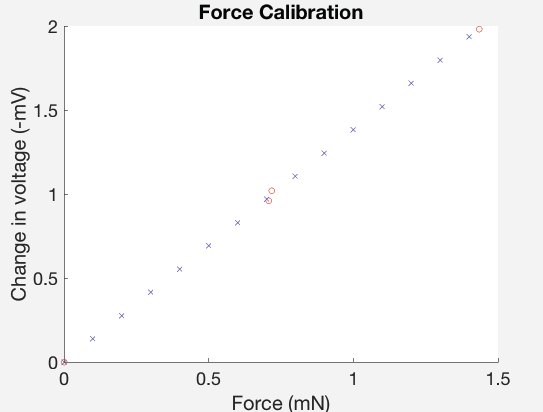
\includegraphics[width = .95\textwidth]{Figures/ForceCal.png}
	\caption{Calibration of force curve. Red circles represent measured changes in voltage for a  set of known forces (using the paperclips and gravity. The blue Xs show the fit line depicting the relationship between change in voltage and force. }
\end{figure}
%Dissection of Frog
\par{}
A decapitated frog was obtained and the heart was exposed via thoracic dissection. A suture was attached to the apex of the heart and tied to the force transducer hook. The hook was oriented parallel to the dissection table. The force transducer was pulled back until the contraction force signal was clearly visible on the recording and oscilloscope without stretching the heart. A ground wire was then connected to one of the pins holding the lower legs of the from. The bipolar electrode was positioned such that it was touching the anterior epicardiaum of the ventricle throughout the contraction. 
%Frank Sterling Test
\par{}
For the first set of tests involving putting the heart under tension the recording electrode was not used. A baseline recording of the contraction force was taken. The dissection tray was then moved farther away from the force probe at 2 mm increments to put the heart under increasing tension. This was repeated until it was deemed that the hear could not be safely stretched any farther. At each distance a 30 second recording was taken. Once this protocol was finished the distance was returned to the starting distance.

%Drug trials
\par{}
The epicardial recording electrode was then placed as described and a 60 second baseline recording from both the force transducer and recording electrode were captured. The heart was then subjected to 9 chemical interventions. For each intervention continuous recordings were taken. During each recording the heart sat at baseline, then 2-4 drops of the chemical of interest was added and the effect was monitored. The chemical of interest was left on the heart for between 60 and 120 seconds. The heart was then washed with room temperature ringers lactate solution. The protocol of chemicals of interest used was as follows: 2 degrees Celsius ringer's solution, 30 mM caffeine, a mystery drug, 0.55 mM calcium chloride, 4.4 mM calcium chloride, 50 $\mu ~M$ epinephrine, 1 mM acetylcholine, 1 mg/mL atropine, and 1~M potassium chloride. Chemicals were used in this order to balance the effect of each and preserve the stability of the preparation.
%Signal processing
\par{}
All signals recorded were saved as .txt documents. A purpose built matlab script was used to extract the signals and save them in a structure format. PFEIFER, a preprocessing framework for electrograms, was used to filter, baseline correct, fiducilize, auto fiducilize, and time align the signals recorded.\cite{MacLeod2018_p} Briefly, the raw signals for each intervention were imported into pfeifer, where a denoising filter was applied. The user was prompted to identify the first heartbeat from the signal by a set of isoelectric points. These isoelectric points were then used to baseline correct the isolated signal. The user was then prompted to fiducilize the first beat. The QRS complex, T wave, and T peak were fiducilized for each intervention. Additionally the X wave and X peak (custom multipurpose fiducials) were used to identify the contraction wave and contraction peak respectivly of the pressure probe. The manually determined fiducials were then used by PFEIFER to automatically detect any remaining heart beats in the input signal and apply the same baseline correction and fiducilization.

\par{}
To further reduce the noise in the epicardial electrical recordings, the autofiducilized beats during the peak of the intervention were signal averaged. This was done by fitting a spline to each beat within the peak of the intervention. An even sampling of 1500 points was taken from each spline and at each time point these beats were averaged to produce the signal averaged beat.

\par{}
The time aligned force transducer recordings were converted to force by multiplying by $m$. For each intervention the contraction force was calculated as the difference between the basal force and the maximum force. Because these signals were baseline corrected this was simply the maximum of the force for each beat. This contraction force for each beat was plotted for each intervention. Additionally the mean contraction force for each intervention was calculated. For each intervention the beginning of the intervention was color coded as green, and the end as pink with each step inbetween being a graded color step from green to gray to pink. This encoding of color to time allowed the pressure curves for an entire intervention to be plotted to show the gradual changes in contraction force.

\par{}
To calculate heart rate for each intervention both the force transducer and electrode recordings were used independently. In each case the time between each fiducilized beat was tracked as the global start of each beat is output from PFEIFER. This resulted in a beat to beat heart rate. Because PFEIFER will occasionally not autofidiculize a beat if it looks too dissimilar from neighboring beats this caused the mean heart rate to sometime be unreliable as missed beats would appear as drastically lowered heart rates between beats. Thus the median calculated heart rate was used for both force transducer and electrode calculated heart rates.

\par{}
For the calculation of the Frank Starling curve the force transducer recordings were processed as described above but baseline correction was omitted to allow for calculation of basal force. For each distance the basal force was found for each beat as the minimum of the force curve and the contraction force as the maximum. These results were plotted together and the relationship was observed.

\section{Results}

%frank Sterling Curve
\par{}
Figure~\ref{fig:FSCurve} shows the results of the Frank Starling stretch protocol. As can be seen increases in stretch lead to both an increase in contraction force and baseline tension. For the distances used the relationship seems to be purely linear.

\par{}
The results of an example fo the post PFEIFER signal averaging are show in Figure~\ref{fig:SignalProcessing}. As can be seen the autofiducilized beats (colored not black) are noisy still despite the denoising filter. However, because they are time aligned by the autofiducilizing process they can be averaged. The resulting averaged beat shows reduced noise while preserving signal morphology. This represents the average beat for th peak of the intervention.

\par{}
The per-intervention results of the heart rate and contractile force calculation are show in Table~\ref{tab:stats}. The median heart rates per intervention as calculated by using either the electrode recordings or the force probe recordings are displayed together. The asterix indicates that the potassium chloride intervention only lasted for two beats. The heart rate and contractile force after this intervention was zero. 

\par{}
The contractile force during each intervention is show in Figure~\ref{fig:ForceGraph}. Hilighted by the arrows and red lines are the intervention time points. B signifies the start of the experiment with the baseline pre-intervention recordings. Each D marker indicates the addition of a drug/chemical. Each W makrer indicates a washout step where the chest was rinsed with room temperature ringer's solution. Of note the D9 (potassium chloride) segment is very short. This is because after potassium chloride was added the heart stopped within two beats and appreciable signals ceased. 

\par{}
The changes in contraction and in the epicardial recording for each intervention are displayed in Figures~\ref{fig:ColdRinger}-\ref{fig:KCL}. In each figure the top pannel shows the change of the force recordings for each fiducialized beat starting from the pre intervention baseline to the addition of drug and the washout. Early beats int he intervention are mapped to be more green while later beats are mapped to be more pink with middle intervention beats being gray. This is especially well depicted in Figure~\ref{fig:CalcHigh} where the force curve starts in green, then increases in amplitude during the middle of the intervention (gray/dark pink) and returns to near baseline green late in the intervention (light pink). Below the force curves are the results of the signal averaged beat for each intervention in red as compared to the initial baseline in black.

\begin{figure}[H]
	\label{fig:FSCurve}
	\centering
	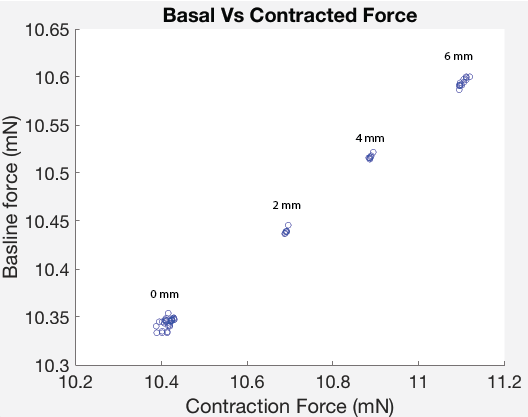
\includegraphics[width = .95\textwidth]{Figures/FSCurve.png}
	\caption{Frank Starling curve. On the x axis is contractile force and on the y axis is relaxed tension. Each cluster represents several beats at that particular stretch length from 0 mm to 6 mm. }
\end{figure}

%Baseline ecg and force curve

%Signal averaged example


\begin{figure}[H]
	\label{fig:SignalProcessing}
	\centering
	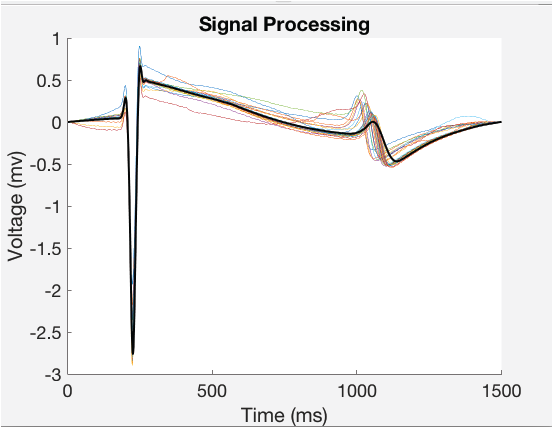
\includegraphics[width = .95\textwidth]{Figures/SP.png}
	\caption{An example fo the beat averaging. Several autofiducilized beats are shown. The beats are averaged into the signal averaged beat (black line) which has greatly reduced noise. }
\end{figure}

%Table of heart rates and contraction forces



\begin{table}[H]
	\centering
	\caption{Numerical results. Mean and Median heart rate are shown as calculated from electrode signals and force probe signals. Mean and Median contractile force is shown.}\label{tab:stats}
	%\rowcolors{2}{gray!25}{white}
	\begin{tabular}{|r r|r|r|}
		\hline
		Drug&&HR (BPM) & Contraction Force (mN) \\
		\hline
		\multirow{2}{*}{Basal}
		&From Electrode & 31.61 &  \\
		&From Force Probe & 31.63 & 0.34 \\
		\hline
		\multirow{2}{*}{Cold Ringers}
		&From Electrode & 26.45&   \\
		&From Force Probe & 24.32 & 0.23 \\
		\hline
		\multirow{2}{*}{Caffeine}
		&From Electrode & 33.25&   \\
		&From Force Probe & 31.01& 0.19 \\
		\hline
		\multirow{2}{*}{Mystery Drug}
		&From Electrode & 34.12 &   \\
		&From Force Probe &33.95 & 0.18  \\
		\hline
		\multirow{2}{*}{Calcium 0.55 mM}
		&From Electrode & 35.21 & \\
		&From Force Probe & 35.04 & 0.14 \\
		\hline
		
		\multirow{2}{*}{Calcium 4.4 mM}
		&From Electrode & 31.25 &   \\
		&From Force Probe & 32.05 & 0.11  \\
		\hline
		
		\multirow{2}{*}{Epinephrine }
		&From Electrode & 33.12 &  \\
		&From Force Probe & 32.65 & 0.09 \\
		\hline
		
		\multirow{2}{*}{Acetylcholine}
		&From Electrode & 25.34 &  \\
		&From Force Probe & 26.53 & 0.02  \\
		\hline
		
		\multirow{2}{*}{Atropine}
		&From Electrode & 30.01 &   \\
		&From Force Probe & 31.25 & 0.07 \\
		\hline
		
		\multirow{2}{*}{Potassium}
		&From Electrode & 30* &   \\
		&From Force Probe & 30.41* & 0.07*  \\
		\hline
		
	\end{tabular}
\end{table}


%Drug Study:
%Force curve


\begin{figure}[H]
	\label{fig:ForceGraph}
	\centering
	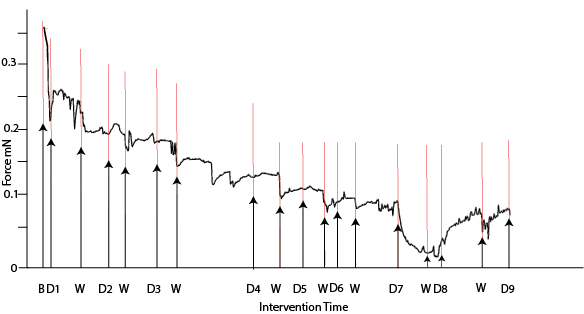
\includegraphics[width = .95\textwidth]{Figures/ForceGraph.png}
	\caption{Graph of changes in contractile force during the experiments. B represents the baseline measurement. Each W represents a time at which the heart was flushed with ringer's lactate solution to wash out. D1 was addition of Cold ringers. D2: caffeine, D3: Mystery drug, D4: 0.55 mM calcium, D5: 4.4 mM calcium. D6: Epinephrine, D7: Acetylcholine, D8: Atropine, D9: Potassium Chloride }
\end{figure}


%Baseline

\begin{figure}[H]
	\label{fig:Baseline}
	\centering
	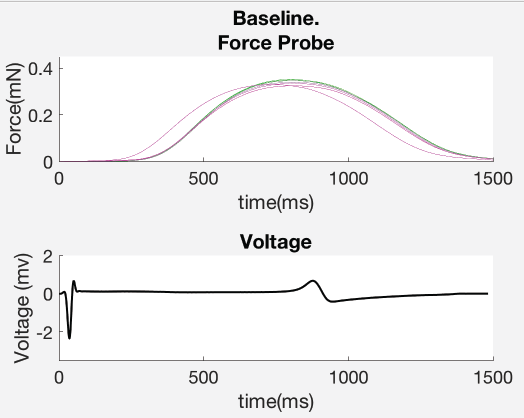
\includegraphics[width = .95\textwidth]{Figures/Baseline.png}
	\caption{Force curve and signal averaged electrical recording.(Top) Force Probe recorded force. The curves progress from green to gray to pink with time. (Bottom) Signal averaged voltage from the ventricles shown in black. }
\end{figure}

%Cold ringers

\begin{figure}[H]
	\label{fig:ColdRinger}
	\centering
	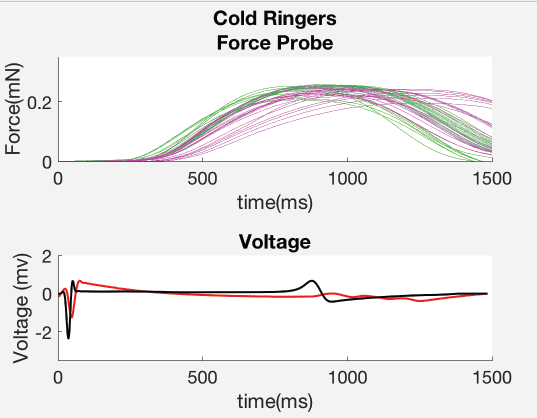
\includegraphics[width = .95\textwidth]{Figures/ColdR.png}
	\caption{Force curve and signal averaged electrical recording.(Top) Force Probe recorded force. The curves progress from green to gray to pink with time. (Bottom) Signal averaged voltage from the ventricles. Baseline signal shown in black, cold ringers signal shown in red. }
\end{figure}

%Caffine
\begin{figure}[H]
	\label{fig:Caffine}
	\centering
	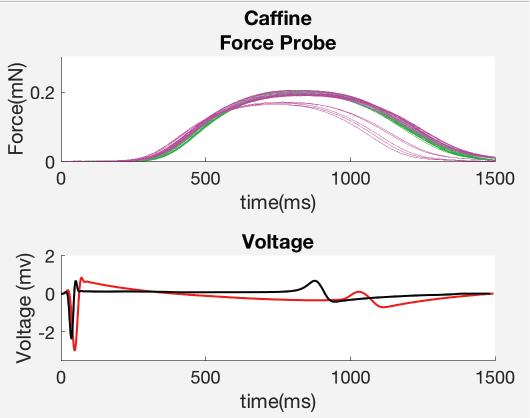
\includegraphics[width = .95\textwidth]{Figures/Caffine.png}
	\caption{Force curve and signal averaged electrical recording.(Top) Force Probe recorded force. The curves progress from green to gray to pink with time. (Bottom) Signal averaged voltage from the ventricles. Baseline signal shown in black, caffeine signal shown in red. }
\end{figure}

%Drug X
\begin{figure}[H]
	\label{fig:Drugx}
	\centering
	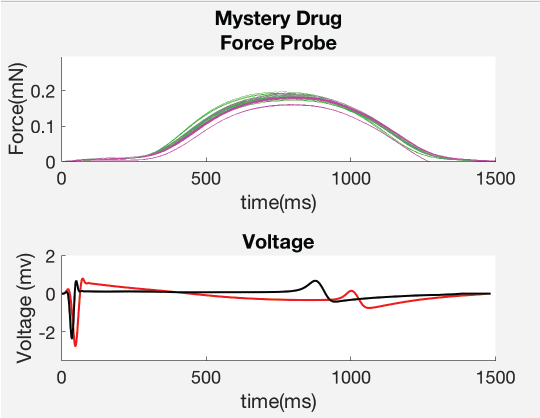
\includegraphics[width = .95\textwidth]{Figures/Drugx.png}
	\caption{Force curve and signal averaged electrical recording.(Top) Force Probe recorded force. The curves progress from green to gray to pink with time. (Bottom) Signal averaged voltage from the ventricles. Baseline signal shown in black, mystery drug signal shown in red. }
\end{figure}
%CaCl2 0.55mM
\begin{figure}[H]
	\label{fig:CalcLow}
	\centering
	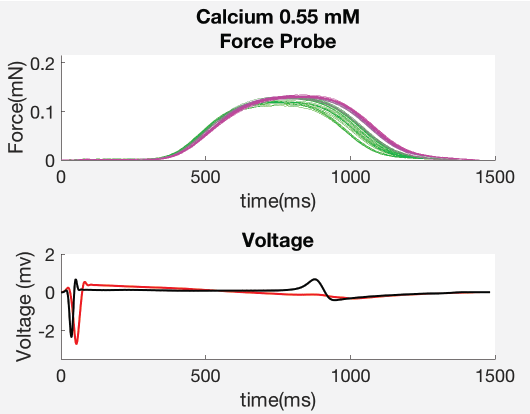
\includegraphics[width = .95\textwidth]{Figures/CalciumLow.png}
	\caption{Force curve and signal averaged electrical recording.(Top) Force Probe recorded force. The curves progress from green to gray to pink with time. (Bottom) Signal averaged voltage from the ventricles. Baseline signal shown in black, 0.55 mM Calcium signal shown in red. }
\end{figure}
%CaCl2 4.4 mM
\begin{figure}[H]
	\label{fig:CalcHigh}
	\centering
	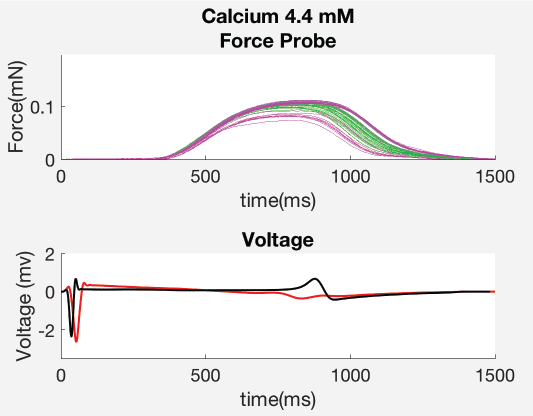
\includegraphics[width = .95\textwidth]{Figures/Calciumhigh.png}
	\caption{Force curve and signal averaged electrical recording.(Top) Force Probe recorded force. The curves progress from green to gray to pink with time. (Bottom) Signal averaged voltage from the ventricles. Baseline signal shown in black, 4.4 mM Calcium signal shown in red. }
\end{figure}
%Epi
\begin{figure}[H]
	\label{fig:Epi}
	\centering
	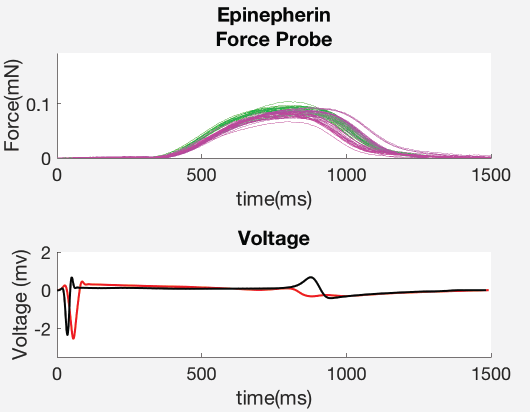
\includegraphics[width = .95\textwidth]{Figures/Epi.png}
	\caption{Force curve and signal averaged electrical recording.(Top) Force Probe recorded force. The curves progress from green to gray to pink with time. (Bottom) Signal averaged voltage from the ventricles. Baseline signal shown in black, epinephrine  signal shown in red. }
\end{figure}
%Ach 1 mM
\begin{figure}[H]
	\label{fig:Ach}
	\centering
	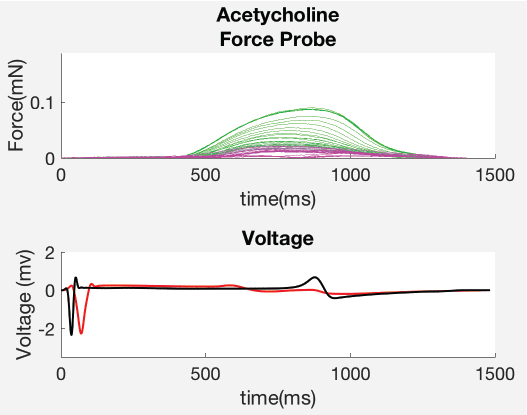
\includegraphics[width = .95\textwidth]{Figures/Ach.png}
	\caption{Force curve and signal averaged electrical recording.(Top) Force Probe recorded force. The curves progress from green to gray to pink with time. (Bottom) Signal averaged voltage from the ventricles. Baseline signal shown in black, acetylcholine signal shown in red. }
\end{figure}
%Atropine
\begin{figure}[H]
	\label{fig:Atropine}
	\centering
	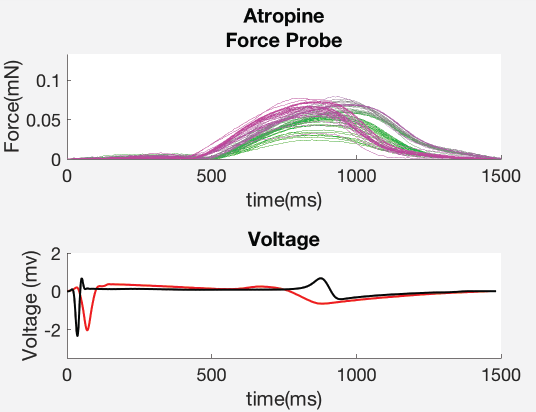
\includegraphics[width = .95\textwidth]{Figures/Atropine.png}
	\caption{Force curve and signal averaged electrical recording.(Top) Force Probe recorded force. The curves progress from green to gray to pink with time. (Bottom) Signal averaged voltage from the ventricles. Baseline signal shown in black, atropine signal shown in red. }
\end{figure}
%KCl
\begin{figure}[H]
	\label{fig:KCL}
	\centering
	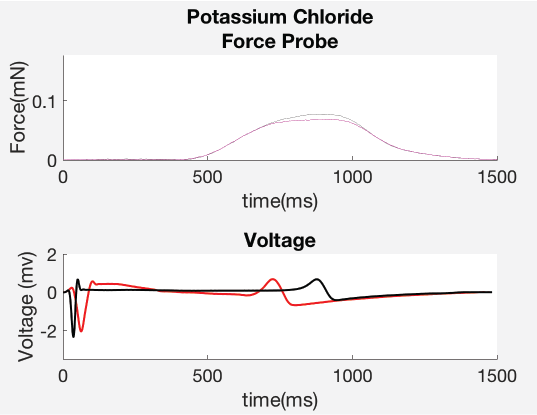
\includegraphics[width = .95\textwidth]{Figures/KCl.png}
	\caption{Force curve and signal averaged electrical recording.(Top) Force Probe recorded force. The curves progress from green to gray to pink with time. (Bottom) Signal averaged voltage from the ventricles. Baseline signal shown in black, potassium signal shown in red. }
\end{figure}
\section{Discussion}
\par{}
The purpose of this lab was to investigate the response of a frog heart's rate and strength of contraction in response to the described interventions. These interventions can be related to various scenarios encountered by a frog heart in different natural states, and thus understanding these responses can inform our understanding of the natural function of a frog heart. 

\par{}
During the Frank Starling stretch test we aimed to simulate the effect of increased venous flow to the heart. Such a situation can occur when the hear rate increases, thus blood flows faster into the heart. This requires that the heart increase its contractile strength to allow it to pump the increased volume of blood. During this intervention we noted that increased stretch resulted not only in increased basal tension, but also increased contractile force, as expected (Figure~\ref{fig:FSCurve}). It is known that this relationship is linear within a certian range but then the contraction force plateaus for any increase in stretch. We were unable to reach this plateau phase as the amount of stretch we exerted on the heart seemed to reach the mechanical limits of our preparation. We did not want to risk ripping the suture out with any further stretching.

\par{}
The remaining interventions replicate scenarios where the phsiology of the heart is affected by various external stimuli. The cold ringer's solution simulates a scenario where the frog encounters a cold environment and its core body temperature begins to drop. During our intervention we see that the heart rate did indeed drop as compared to the basal heart rate (Table~\ref{tab:stats}). The contraction force also appears to be lower than the basal contraction force, however we see another drop in contraction force during th ecolld ringer's washout(Figure~\ref{fig:ForceGraph}). However it can be noted that regardless of the interventions the contractile force decayed sharply over time due to instability of the preparation. Once beheaded it was only a matter of time before the heart stopped altogether no matter which interventions we performed. As such all changes in contractile strength are comfounded by this decay in model stability. However for the cold ringer's intervention we do see that, as the heart rate slows the contractions also slow, and then recover with washout as seen in Figure~\ref{fig:ColdRinger}.
\par{}
The caffeine intervention can shed light into the effects of caffeine on hearts in general. Contrary to expectations the heart rate increase seen with caffeine was moderate (Table~\ref{tab:stats}). Minimal changes were seen in the contractile force (Figure~\ref{fig:ForceGraph}). This minimal affect could be attributed to the fact that caffeine is typically delivered via the blood rather than extracellularly. As such perhaps only a small amount of the caffeine actually was able to affect the cells of the heart.

\par{}
The mystery drug represents a clinical scenario where a paitent is exposed to some cardomodulatory toxin or other substance. By observing its effect on the heart we can predict its mechanism of action. It appears that the drug did not affect the contractile force (figure~\ref{fig:Drugx}) but it did increase the heart rate (Table~\ref{tab:stats}). The only other intervention with a similar effect was epinephrine. This suggests that perhaps the two act through a similar mechanism. Based on these data it would seem that the mystery drug is some sort of stimulant that causes an increase in heart rate.

\par{}
The two calcium interventions represent scenarios where calcium handling is effected in the heart. In the case of the 0.55 mM calcium something, such as an ion channel mutation or other deficiency, has caused low extracellular calcium. We expect that this should  result in a decrease in contractility. However from our data we see no major decrease in contractility, but rather an increase in heart rate (Table~\ref{tab:stats}, Figure~\ref{fig:ForceGraph},Figure~\ref{fig:CalcLow}).Decreased extracellular calcium results in a loss of the plateau phase as this is primarily driven by inward calcium flow. Thus the cells can repolarize more quickly and thus are able to excite sooner, resulting in an increased heart rate. Notably we also see that the T wave (a section of the signal associated with repolarization) of the low calcium intervention was almost non extant (Figure~\ref{fig:CalcLow}).
\par{}
In the case of the 4.4 mM calcium this represents the opposite scenario where calcium in the extracellular space is higher than usual. In this case we would expect an increase in contractile strength as a larger influx of calcium would occur during the cardiac action potential. This would result in a greater amount of sarcoplasmic reticulum calcium release and thus a stronger contraction via a larger calcium transient. We do see a marginal increase in contractility during the intervention followed by a decrease at the washout (Figure~\ref{fig:CalcHigh}).
\par{}
Int he case of the epinephrine intervention this represents  stimulus from the sympathetic nervous system. Often this is associated with the fight or flight response such as when the frog becomes frightened or in pain. sympathetic stimulation of the heart causes it to beat faster to provide blood to the body so that it can be ready to, as the phrase suggests, fight or flee. During this intervention we saw an increase in heart rate over basal levels and no discernible pattern of change in contractile force as expected (Table~\ref{tab:stats}, Figure~\ref{fig:ForceGraph},Figure~\ref{fig:Epi}).

\par{}
Acetycholine is the primary acting molecule of the parasympathetic nervous system. This intervention represents parasympathetic stimulation, as would happen when the frog begins to relax or perhaps goes to sleep. In such a scenario the heart slows to conserve energy. In our intervention addition of just 1 mM of acetylcholine nearly stopped the heart. As can be seen in Figure~\ref{fig:Ach}, and Figure~\ref{fig:Ach} the contractile force dropped near to zero quickly, however the electrical activity of the heart persisted. The heart rate dropped as expected (Table~\ref{tab:stats}).
\par{}
Atropine is used clinically to rescue low hear rate, thus as expected the addition of atropine resulted in a gradual increased heart rate and contractility (Table~\ref{tab:stats}, Figure~\ref{fig:ForceGraph},Figure~\ref{fig:Atropine}). After the washout of the acetocholine intervention the heart rate remained depressed, possibly due to poor washout, latent effects of the acetylcholine, or declining stability of the preparation. Despite this the addition of acetylcholine returned the contractility and heart rate to nearly pre acetylcholine levels.

\par{}
The final intervention was 1 M potassium chloride. This is a concentration nearly 1000 times more concentrated than the ringer's solution potassium levels. This scenario represents severe mishandling of extracellular potassium which can arise in some disease states or when the potassium pumps no longer function. In these scenarios the resting membrane potential rises quickly as potassium is the main driver of membrane potential. This results in the inability of sodium channels to de-inactivate (which requires a low negative membrane potential of around - 30 mV). Thus sodium channels can no longer activate and thus no further action potentials can arise. When we added potassium chloride to the heart it stopped within two beats, demonstrating this principle. The intervention was not long enough to see any gradual changes in contractility or heart rate. Marginal electrical activity continued to occur withint he tissue of the heart but it was within the noise floor of our recording.

\par{}
Through these interventions we have demonstrated the response of the frog heart to physical and chemical changes in its environment. These various changes represent both natural and disease state situations experienced by the heart and allow for the investigation of the development of these changes within the heart. Notably these results are confounded by the instability of the preparation. Because the frog is beheaded it constantly bleeds out, resulting in eventual loss of blood pressure, and a steady decline in cardiac function throughout the experiment.

%%%%%%%%%%%%%%%%%% Correct Bibliography Style

\bibliography{C:/Users/Jake/Documents/library}
\bibliographystyle{IEEEtran}


\end{document}








